% ==============================================================================
% Final Journal Figure Captions for SecChaos-RL
% Target Journal: Software: Practice and Experience (Wiley)
% ==============================================================================

% ------------------------------------------------------------------------------
% Figure 1: Overall SecChaos-RL Closed-Loop Methodology & System Architecture
% ------------------------------------------------------------------------------
\begin{figure*}[!t]
\centering
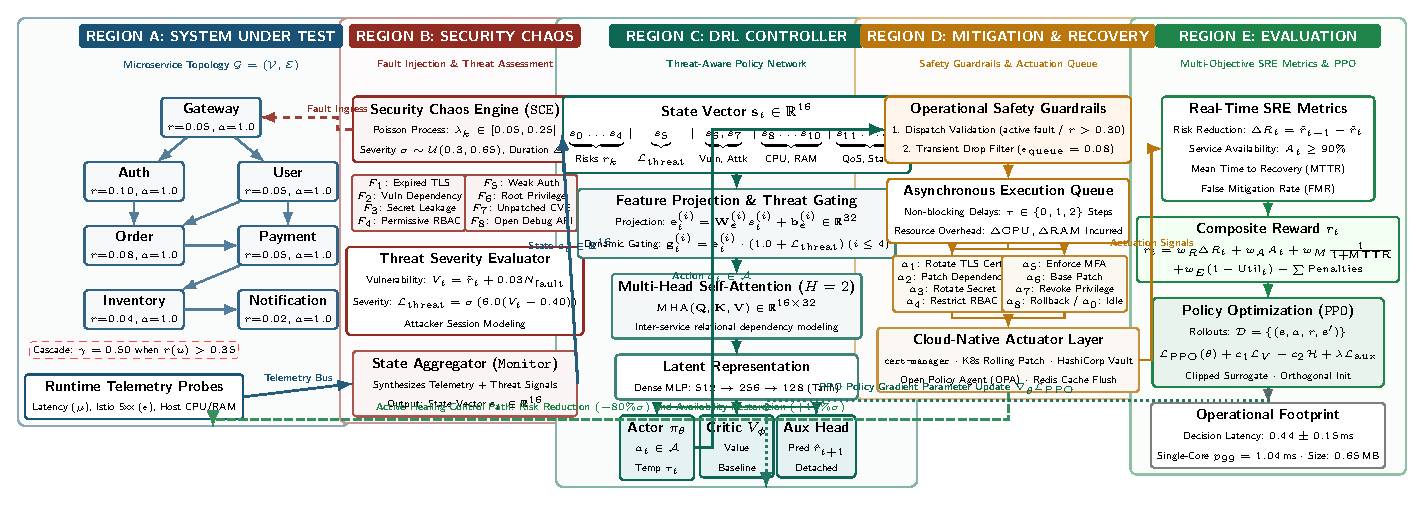
\includegraphics[width=\textwidth]{figure_redesign/secchaos_main_methodology.pdf}
\caption{Overall SecChaos-RL closed-loop resilience engineering framework. The workflow proceeds through five coordinated functional regions: 
(Region~A) The target microservice system structured as a directed acyclic dependency graph $\mathcal{G} = (\mathcal{V}, \mathcal{E})$ with runtime telemetry monitoring; 
(Region~B) The Security Chaos Engine injecting standardized stochastic faults ($F_1$--$F_8$, Poisson arrival $\lambda_k \in [0.05, 0.25]$) alongside continuous logistic threat severity evaluation ($\mathcal{L}_{\mathrm{threat}}$); 
(Region~C) The threat-aware deep reinforcement learning controller featuring linear state feature projection, threat-aware feature gating, multi-head self-attention ($H=2$), and three decoupled output heads (actor policy $\pi_\theta$ with adaptive temperature $\tau_t$, critic baseline $V_\phi$, and auxiliary risk prediction head $\hat{\mathbf{r}}_{t+1}$); 
(Region~D) Operational safety guardrails (dispatch validation and transient queue drop filter $\epsilon_{\mathrm{queue}} = 0.08$), asynchronous execution queue ($\tau \in \{0, 1, 2\}$), and cloud-native remediation actuators delivering active service healing (reducing targeted service risk by $80\%\sigma$ and restoring availability by $+15\%\sigma$); and 
(Region~E) Multi-objective performance evaluation tracking service availability, recovery time (MTTR), security risk reduction, and false mitigation rate (FMR), driving PPO policy gradient updates ($\nabla_\theta \mathcal{L}_{\mathrm{PPO}}$) through the closed learning loop. 
Abbreviations: DAG: Directed Acyclic Graph; DRL: Deep Reinforcement Learning; FMR: False Mitigation Rate; MTTR: Mean Time to Recovery; PPO: Proximal Policy Optimization; SCE: Security Chaos Engineering.}
\label{fig:framework_architecture}
\end{figure*}

% ------------------------------------------------------------------------------
% Figure 2: Threat-Aware Neural Network Policy Architecture
% ------------------------------------------------------------------------------
\begin{figure*}[!t]
\centering
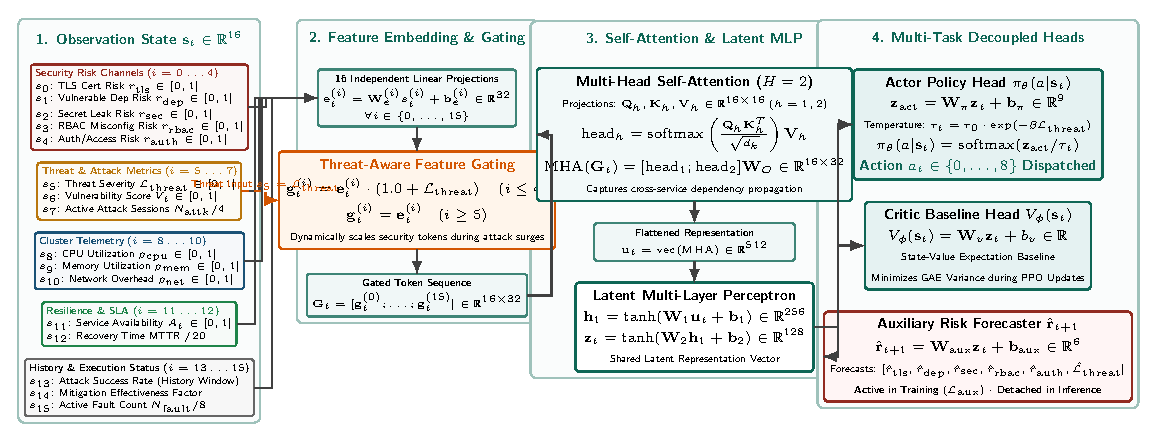
\includegraphics[width=0.95\textwidth]{figure_redesign/secchaos_network_architecture.pdf}
\caption{Threat-aware deep neural policy network architecture. 
(1) Standardized 16-dimensional observation vector $\mathbf{s}_t \in \mathbb{R}^{16}$ categorized into security risks ($s_0$--$s_4$), threat dynamics ($s_5$--$s_7$), cluster resource telemetry ($s_8$--$s_{10}$), resilience QoS ($s_{11}$--$s_{12}$), and execution history ($s_{13}$--$s_{15}$); 
(2) Independent linear feature projection ($\mathbf{e}_t^{(i)} \in \mathbb{R}^{32}$) coupled with multiplicative threat-aware gating ($\mathbf{g}_t^{(i)} = \mathbf{e}_t^{(i)} \cdot (1 + \mathcal{L}_{\mathrm{threat}})$ for $i \le 4$); 
(3) Two-head self-attention layer ($H=2, d_k=16$) capturing topological inter-service failure dependencies, followed by flattening and shared dense representation layers ($512 \to 256 \to 128$, Tanh); and 
(4) Multi-task decoupled output heads: Actor policy $\pi_\theta(a|\mathbf{s}_t)$ with threat-adaptive temperature $\tau_t = \tau_0 \exp(-\beta \mathcal{L}_{\mathrm{threat}})$, Critic state-value baseline $V_\phi(\mathbf{s}_t)$, and Auxiliary next-step risk predictor $\hat{\mathbf{r}}_{t+1} \in \mathbb{R}^6$ (active during PPO policy training and detached during runtime inference). 
Abbreviations: MHA: Multi-Head Attention; MLP: Multi-Layer Perceptron; QoS: Quality of Service.}
\label{fig:network_architecture}
\end{figure*}

% ------------------------------------------------------------------------------
% Figure 3: Quantitative Resilience Benchmarking Across 30 Seeds (RQ1)
% ------------------------------------------------------------------------------
% \begin{figure*}[!t]
% \centering
% 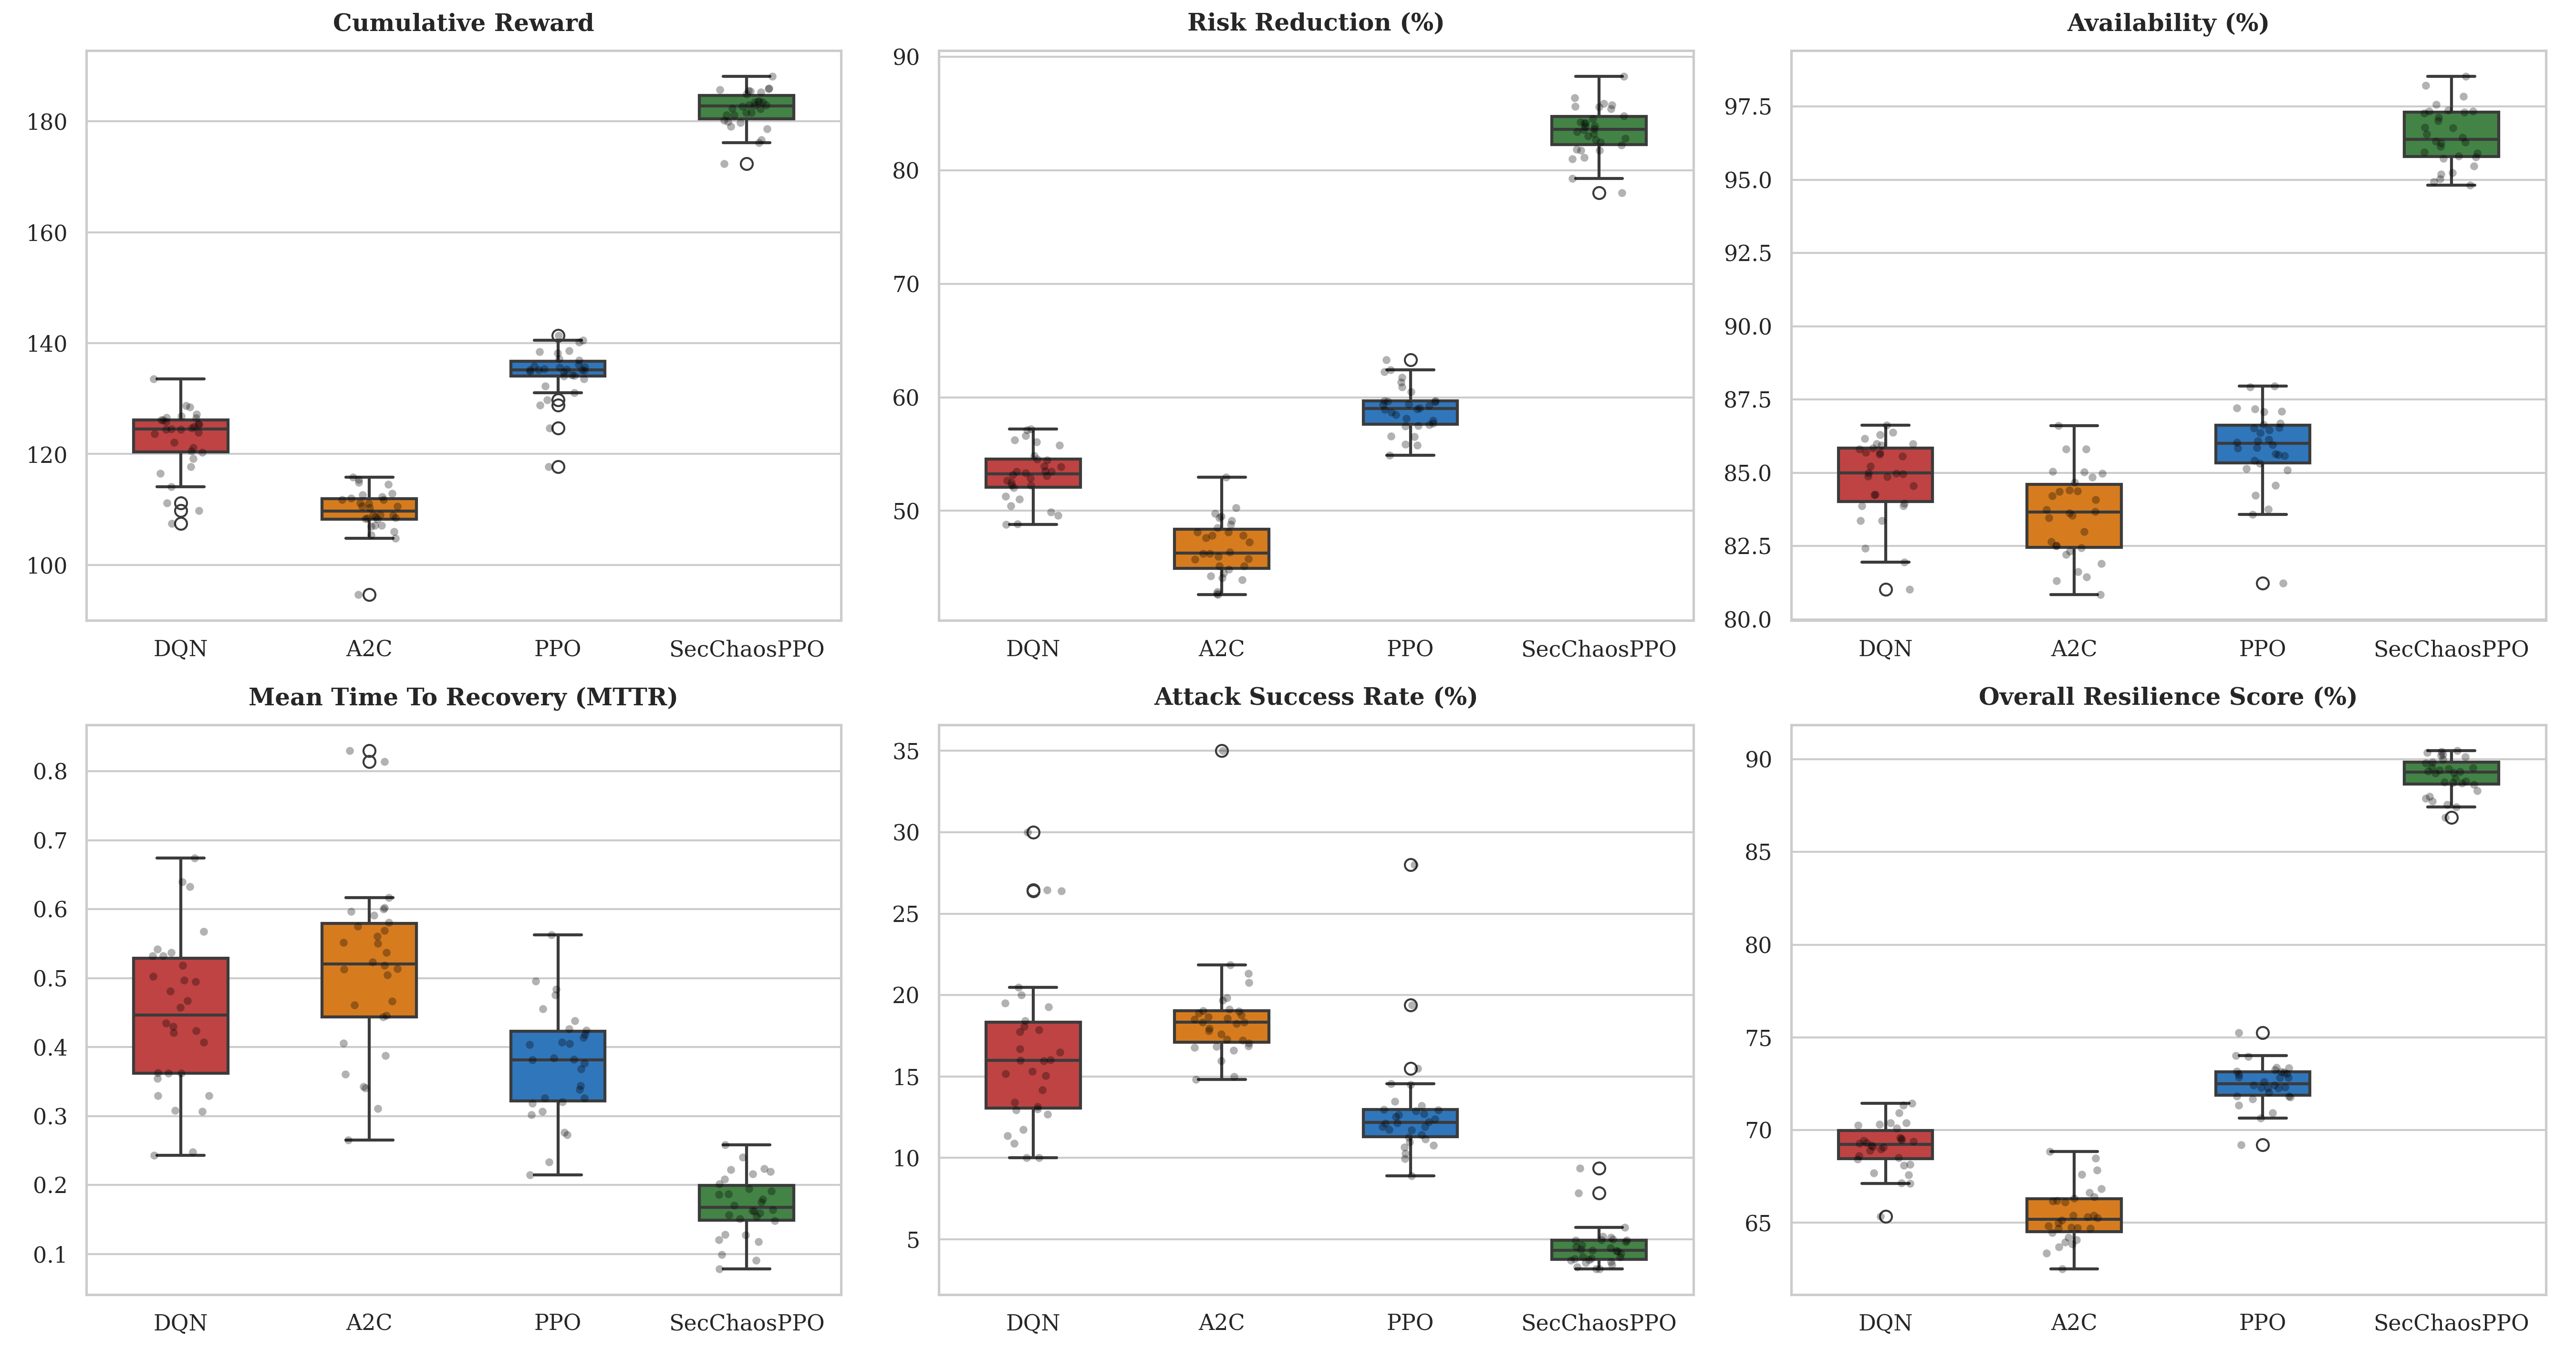
\includegraphics[width=0.92\textwidth]{figs/resilience_benchmarking.png}
% \caption{Comprehensive quantitative resilience benchmarking across 30 independent random seeds under multi-stage security chaos: Distributions of Security Risk Reduction (\%), Service Availability (\%), Mean Time to Recovery (MTTR in operational steps), Attack Success Rate (ASR, \%), False Mitigation Rate (FMR, \%), and Composite Resilience Score (\%) across eight evaluated control policies. Boxplots display median, interquartile range (IQR), and full sample ranges.}
% \label{fig:resilience_benchmarking}
% \end{figure*}

% ------------------------------------------------------------------------------
% Figure 4: Pareto Trade-off Between Risk Reduction and Availability (RQ2)
% ------------------------------------------------------------------------------
% \begin{figure}[!htbp]
% \centering
% \includegraphics[width=\columnwidth, keepaspectratio]{figs/pareto_tradeoff.png}
% \caption{Empirical Pareto frontier between Security Risk Reduction and Service Availability across 30 random seeds, illustrating the operational boundary separating deterministic rule-based heuristics (high local risk reduction, severe action churn) from autonomous reinforcement learning policies (balanced availability preservation, lower FMR).}
% \label{fig:pareto_tradeoff}
% \end{figure}

% ------------------------------------------------------------------------------
% Figure 5: Ablation Study Across Successive Architectural Stages (RQ3)
% ------------------------------------------------------------------------------
% \begin{figure*}[!t]
% \centering
% \includegraphics[width=0.88\textwidth]{figs/ablation_study.png}
% \caption{Ablation analysis across successive architectural stages over 30 independent seeds: (Stage 1) Baseline PPO; (Stage 2) +Multi-Objective Resilience Reward; (Stage 3) +Multi-Head Self-Attention; (Stage 4) +Auxiliary Risk Prediction Head; and (Stage 5) Full SecChaos-RL Framework with Threat-Adaptive Exploration. Error bars represent 95\% confidence intervals.}
% \label{fig:ablation_study}
% \end{figure*}

% ------------------------------------------------------------------------------
% Figure 6: Training Convergence Trajectories Across Curriculum Stages (RQ4)
% ------------------------------------------------------------------------------
% \begin{figure}[!htbp]
% \centering
% 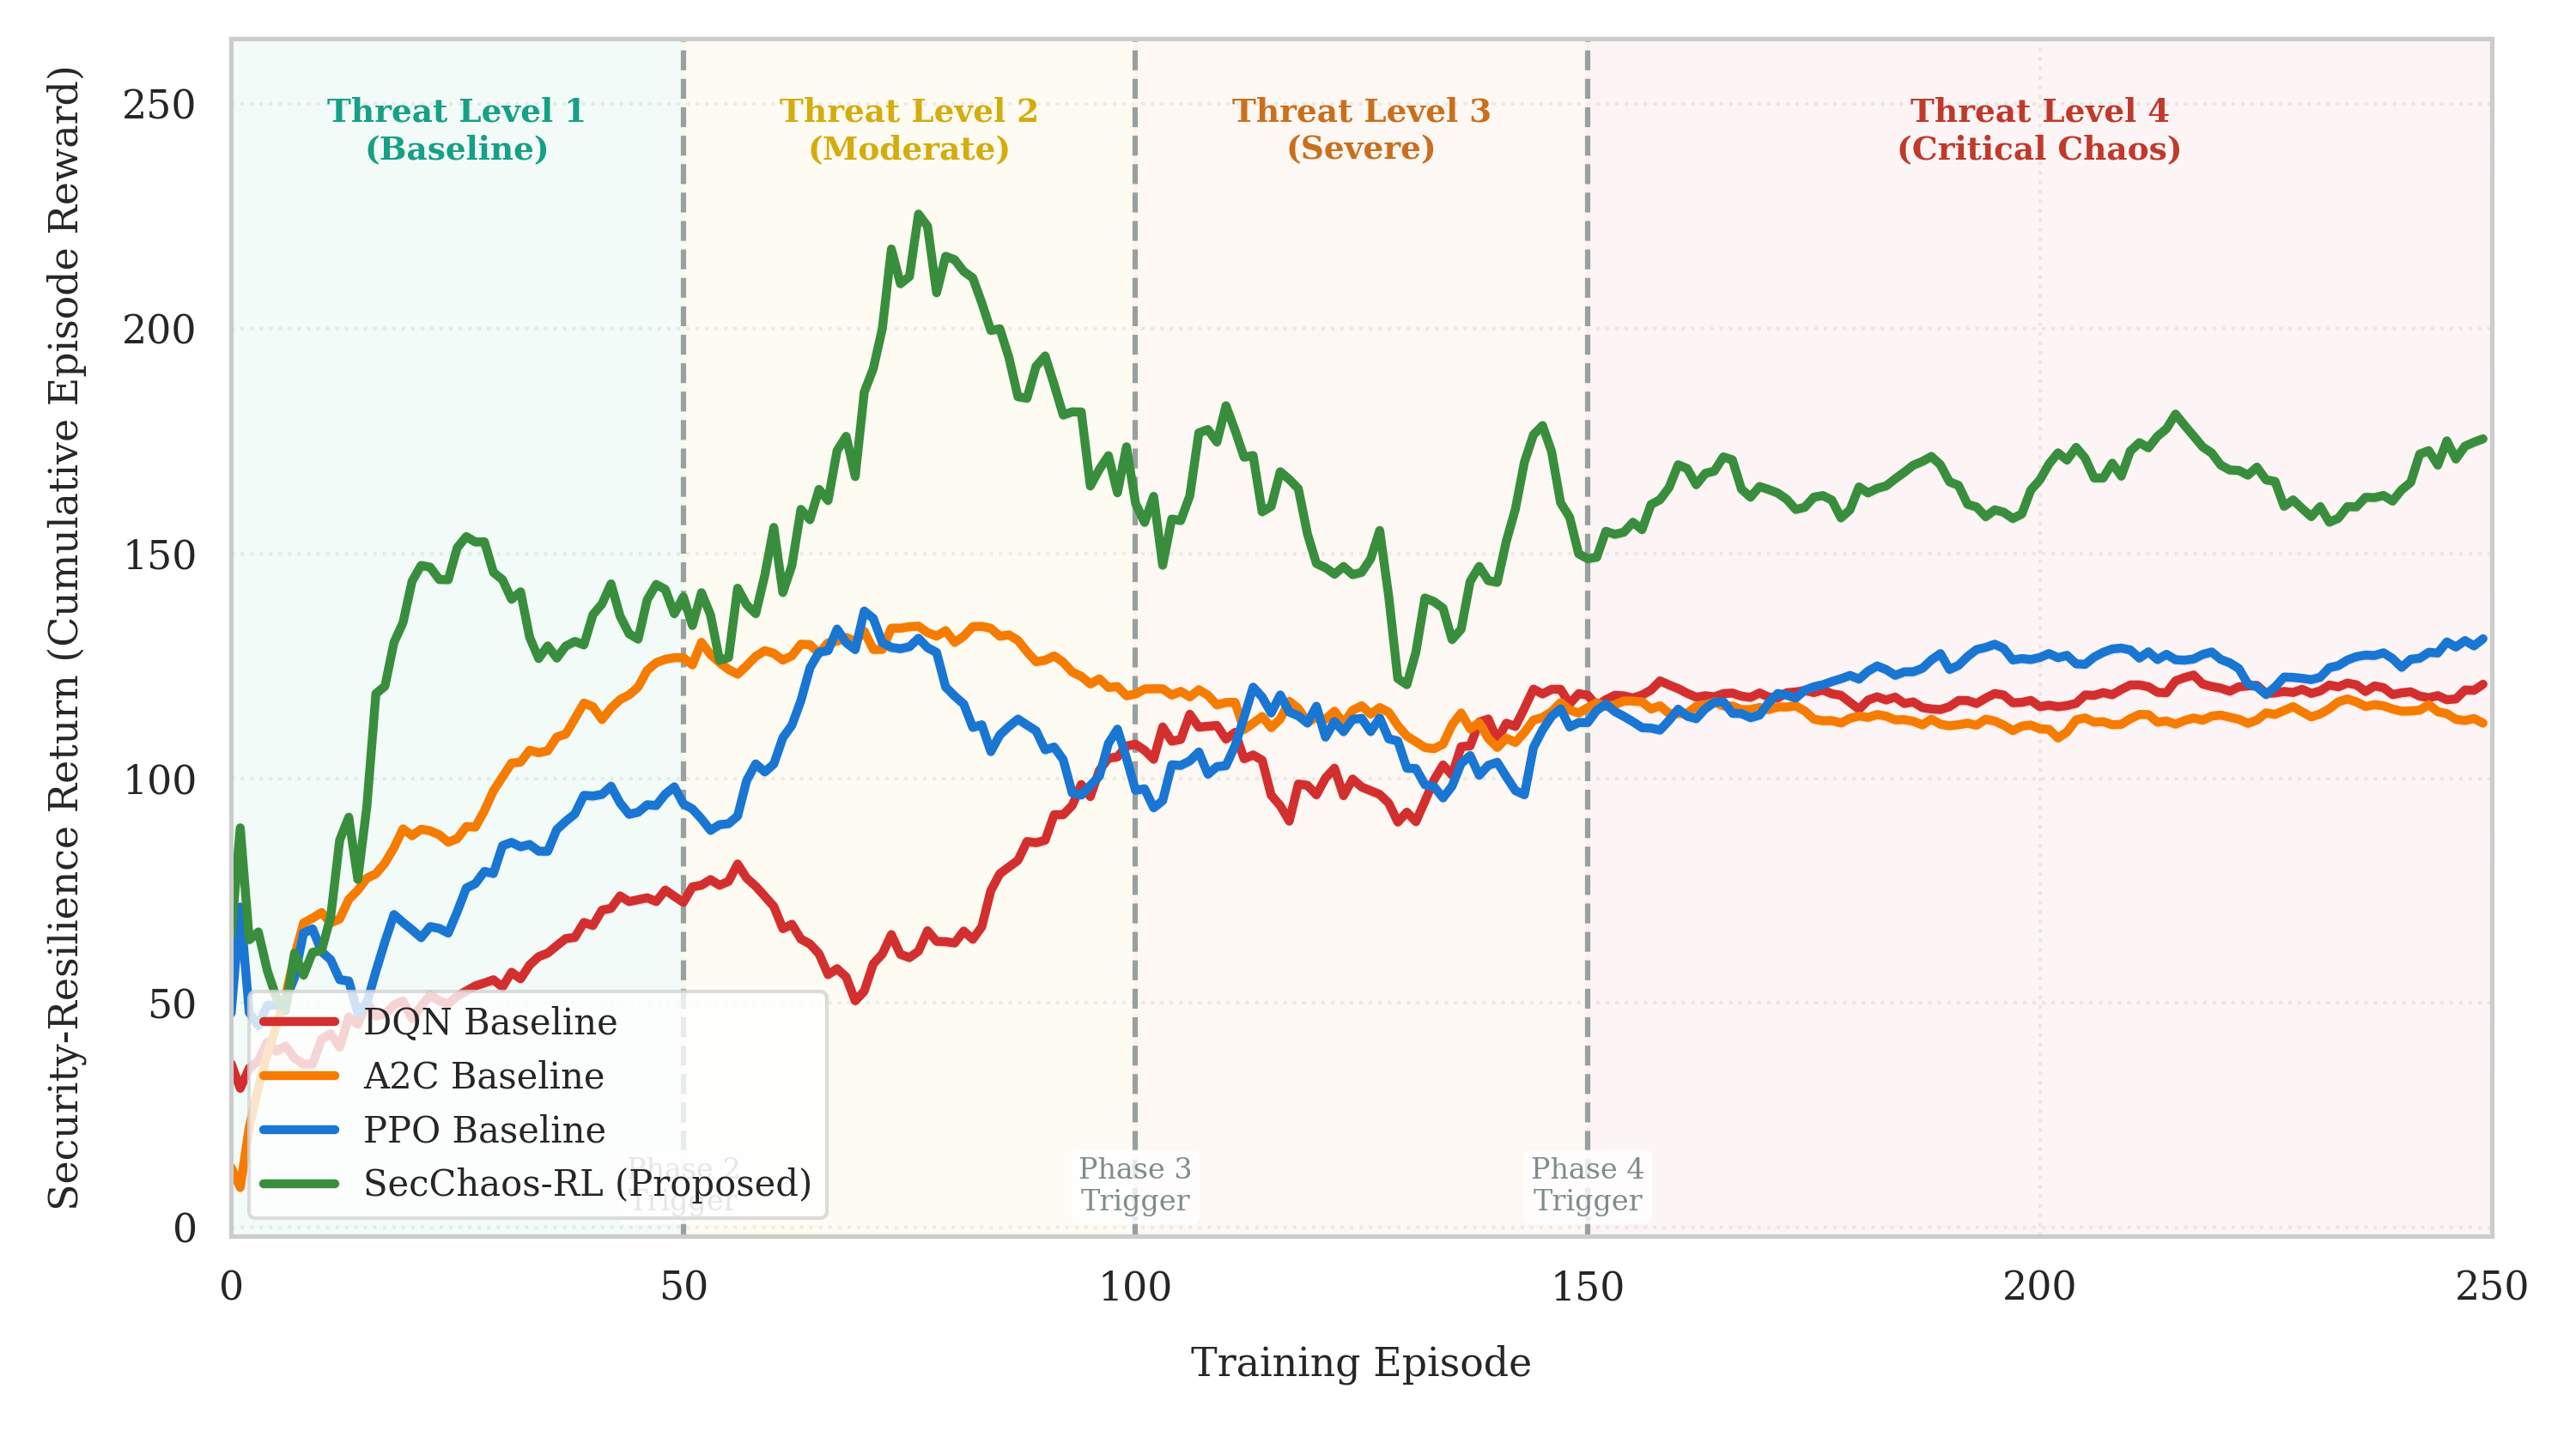
\includegraphics[width=\columnwidth, keepaspectratio]{figs/learning_curves.png}
% \caption{Training convergence trajectories across 30 random seeds through curriculum progression (Stages 0--3) with 95\% confidence intervals, showing cumulative episode return, policy entropy decay, and auxiliary risk prediction loss stabilization.}
% \label{fig:learning_curves}
% \end{figure}
